\begin{center}
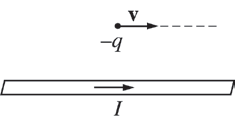
\includegraphics[scale=0.5]{images/img-008-022.png}
\end{center}

% Multiple Choice Question 30
\begin{questions}\setcounter{question}{29}\question
A negative charge $-q$ is moving with a velocity $\mathbf{v}$ to the right, parallel to a wire that is carrying a current $I$ to the right, as shown above. The direction of the force on the charge due to the magnetic field produced by the wire is

\begin{choices}
\choice toward the top of the page
\choice toward the bottom of the page
\choice out of the page
\choice into the page
\choice toward the left
\end{choices}\end{questions}

